% 图 8.9 (a) 均匀自旋链：M 形自旋子连续谱 + 链示意（J、晶格常数 a）
%        (b) 交替链（二聚化）：有隙 V 形带 + 链示意（J1/J2、单胞 2a）
\documentclass[tikz,border=5pt]{standalone}
\usetikzlibrary{arrows.meta,patterns}
\usepackage{amsmath}
\usepackage{bm}
\usepackage{fontspec}
\setmainfont{Times New Roman}
\pgfdeclarepatternformonly{speckle}{\pgfpointorigin}{\pgfpoint{5pt}{5pt}}{\pgfpoint{5pt}{5pt}}{
  \pgfsetcolor{black!72}
  \pgfpathcircle{\pgfpoint{0.8pt}{1.2pt}}{0.55pt}
  \pgfpathcircle{\pgfpoint{2.7pt}{3.5pt}}{0.6pt}
  \pgfpathcircle{\pgfpoint{4.2pt}{0.7pt}}{0.5pt}
  \pgfpathcircle{\pgfpoint{1.7pt}{4.4pt}}{0.45pt}
  \pgfpathcircle{\pgfpoint{3.9pt}{2.3pt}}{0.4pt}
  \pgfusepath{fill}}
\begin{document}
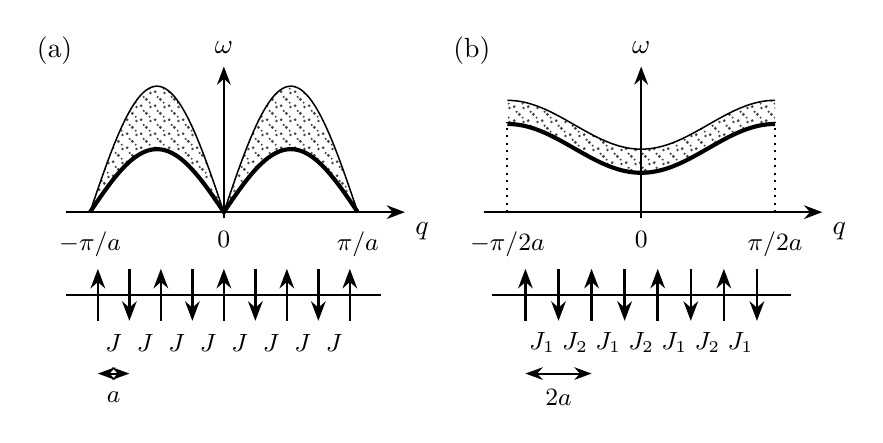
\begin{tikzpicture}[line width=0.8pt,>=Stealth,
  chainar/.style={line width=0.9,{Stealth[length=2.4mm,width=1.8mm]}-{Stealth[length=2.4mm,width=1.8mm]}}]
% ================= (a) uniform chain =================
\begin{scope}[shift={(0,0)}]
  \node at (-2.15,2.05) {(a)};
  % continuum band
  \fill[pattern=speckle]
    plot[domain=-180:180,samples=121,smooth] ({1.7*\x/180},{0.80*abs(sin(\x))})
    -- plot[domain=180:-180,samples=121,smooth] ({1.7*\x/180},{1.60*abs(sin(\x))})
    -- cycle;
  \draw[line width=1.5,domain=-180:180,samples=121,smooth]
    plot ({1.7*\x/180},{0.80*abs(sin(\x))});
  \draw[line width=0.55,domain=-180:180,samples=121,smooth]
    plot ({1.7*\x/180},{1.60*abs(sin(\x))});
  % axes
  \draw[->] (-2.0,0) -- (2.3,0) node[below right]{$q$};
  \draw[->] (0,-0.08) -- (0,1.85) node[above=1pt]{$\omega$};
  \node[below] at (-1.7,-0.12) {\small $-\pi/a$};
  \node[below] at (0,-0.12) {\small $0$};
  \node[below] at (1.7,-0.12) {\small $\pi/a$};
  % spin chain
  \draw[line width=0.7] (-2.0,-1.05) -- (2.0,-1.05);
  \foreach \i in {0,...,8}{
    \pgfmathsetmacro{\x}{-1.6+\i*0.4}
    \pgfmathtruncatemacro{\d}{mod(\i,2)}
    \ifnum\d=0
      \draw[->,line width=0.9] (\x,-1.38) -- (\x,-0.72);
    \else
      \draw[->,line width=0.9] (\x,-0.72) -- (\x,-1.38);
    \fi}
  \foreach \i in {0,...,7}{
    \pgfmathsetmacro{\x}{-1.4+\i*0.4}
    \node at (\x,-1.66) {\small $J$};}
  \draw[{Stealth[length=2.2mm,width=1.6mm]}-{Stealth[length=2.2mm,width=1.6mm]},line width=0.7]
    (-1.6,-2.05) -- (-1.2,-2.05);
  \node at (-1.4,-2.35) {\small $a$};
\end{scope}
% ================= (b) alternating (dimerized) chain =================
\begin{scope}[shift={(5.3,0)}]
  \node at (-2.15,2.05) {(b)};
  % gapped V-shaped band
  \fill[pattern=speckle]
    plot[domain=-180:180,samples=121,smooth] ({1.7*\x/180},{0.50+0.31*(1-cos(\x))})
    -- plot[domain=180:-180,samples=121,smooth] ({1.7*\x/180},{0.80+0.31*(1-cos(\x))})
    -- cycle;
  \draw[line width=1.5,domain=-180:180,samples=121,smooth]
    plot ({1.7*\x/180},{0.50+0.31*(1-cos(\x))});
  \draw[line width=0.55,domain=-180:180,samples=121,smooth]
    plot ({1.7*\x/180},{0.80+0.31*(1-cos(\x))});
  % zone boundary dotted lines
  \draw[dotted,line width=0.7] (-1.7,0) -- (-1.7,1.15);
  \draw[dotted,line width=0.7] (1.7,0) -- (1.7,1.15);
  % axes
  \draw[->] (-2.0,0) -- (2.3,0) node[below right]{$q$};
  \draw[->] (0,-0.08) -- (0,1.85) node[above=1pt]{$\omega$};
  \node[below] at (-1.7,-0.12) {\small $-\pi/2a$};
  \node[below] at (0,-0.12) {\small $0$};
  \node[below] at (1.7,-0.12) {\small $\pi/2a$};
  % spin chain with alternating J1, J2
  \draw[line width=0.7] (-1.9,-1.05) -- (1.9,-1.05);
  \foreach \i in {0,...,7}{
    \pgfmathsetmacro{\x}{-1.47+\i*0.42}
    \pgfmathtruncatemacro{\d}{mod(\i,2)}
    \ifnum\d=0
      \draw[->,line width=0.9] (\x,-1.38) -- (\x,-0.72);
    \else
      \draw[->,line width=0.9] (\x,-0.72) -- (\x,-1.38);
    \fi}
  \foreach \i in {0,...,6}{
    \pgfmathsetmacro{\x}{-1.26+\i*0.42}
    \pgfmathtruncatemacro{\d}{mod(\i,2)}
    \ifnum\d=0
      \node at (\x,-1.66) {\small $J_1$};
    \else
      \node at (\x,-1.66) {\small $J_2$};
    \fi}
  \draw[{Stealth[length=2.2mm,width=1.6mm]}-{Stealth[length=2.2mm,width=1.6mm]},line width=0.7]
    (-1.47,-2.05) -- (-0.63,-2.05);
  \node at (-1.05,-2.35) {\small $2a$};
\end{scope}
\end{tikzpicture}
\end{document}
